
\documentclass[dvipdfmx]{standalone}
\usepackage[T1]{fontenc}
\usepackage{newtxtext, newtxmath}

\usepackage{tikz}
\usetikzlibrary{matrix}

\begin{document}
  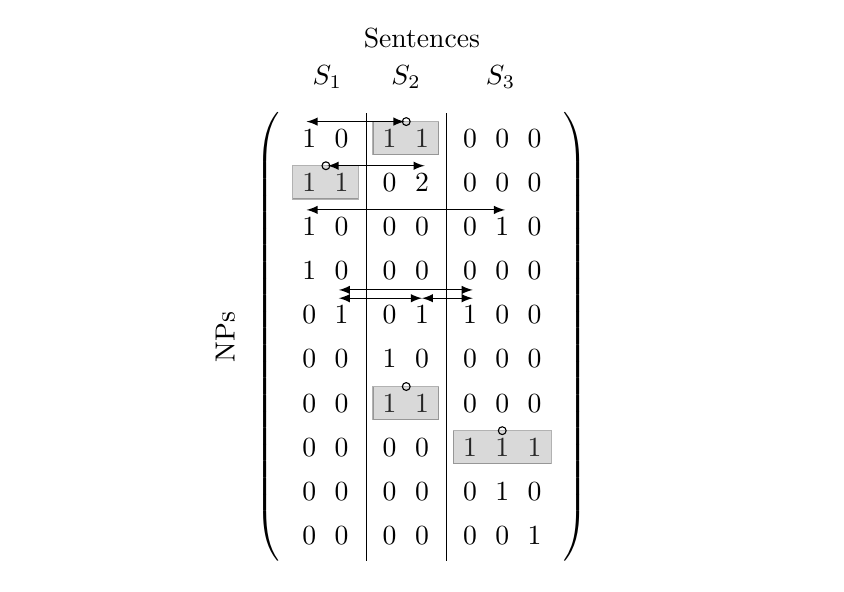
\begin{tikzpicture}
    \tikzset{top/.style={yshift=0.6em}}
    \tikzset{top left/.style={xshift=-0.6em, yshift=0.6em}}
    \tikzset{top right/.style={xshift=0.6em, yshift=0.6em}}
    \tikzset{bottom left/.style={xshift=-0.6em,  yshift=-0.6em}}
    \tikzset{bottom right/.style={xshift=0.6em,  yshift=-0.6em}}

    % centering
    \draw [opacity=0.0] (-5,0) -- (5,0);

    % matrix
    \matrix (matrix) [matrix of math nodes, left delimiter=(, right delimiter=), row sep=1mm]
    {
    1 & 0 &[2mm] 1 & 1 &[2mm] 0 & 0 & 0 \\
    1 & 1 &      0 & 2 &      0 & 0 & 0 \\
    1 & 0 &      0 & 0 &      0 & 1 & 0 \\
    1 & 0 &      0 & 0 &      0 & 0 & 0 \\
    0 & 1 &      0 & 1 &      1 & 0 & 0 \\
    0 & 0 &      1 & 0 &      0 & 0 & 0 \\
    0 & 0 &      1 & 1 &      0 & 0 & 0 \\
    0 & 0 &      0 & 0 &      1 & 1 & 1 \\
    0 & 0 &      0 & 0 &      0 & 1 & 0 \\
    0 & 0 &      0 & 0 &      0 & 0 & 1 \\
    };

    % vertical line
    \coordinate (sec1 end top)    at ([shift={(0.9em, 0.9em)}]matrix-1-2);
    \coordinate (sec1 end bottom) at ([shift={(0.9em,-0.9em)}]matrix-10-2);
    \coordinate (sec2 end top)    at ([shift={(0.9em, 0.9em)}]matrix-1-4);
    \coordinate (sec2 end bottom) at ([shift={(0.9em,-0.9em)}]matrix-10-4);
    \draw[black] (sec1 end top) -- (sec1 end bottom);
    \draw[black] (sec2 end top) -- (sec2 end bottom);

    % text: sentences
    \pgftransformyshift{3.8cm}
    \pgftext{Sentences}
    % text: S1, S2, S3
    \pgftransformyshift{-0.5cm}
    \pgftransformxshift{-1.2cm}
    \pgftext{$S_1$}
    \pgftransformxshift{1.0cm}
    \pgftext{$S_2$}
    \pgftransformxshift{1.2cm}
    \pgftext{$S_3$}
    \pgftransformreset

    % text: NPs
    \pgftransformrotate{90}
    \pgftransformyshift{2.5cm}
    \pgftext{NPs}
    \pgftransformreset

    % cluster
    \tikzset{cluster/.style={fill=black!50!white, opacity=0.3}}
    \draw[cluster] ([top left]matrix-1-3) rectangle ([bottom right]matrix-1-4);
    \draw[cluster] ([top left]matrix-2-1) rectangle ([bottom right]matrix-2-2);
    \draw[cluster] ([top left]matrix-7-3) rectangle ([bottom right]matrix-7-4);
    \draw[cluster] ([top left]matrix-8-5) rectangle ([bottom right]matrix-8-7);

    % cluster centoroid points
    \tikzset{centroid/.style={circle, draw=black, inner sep=1pt}}
    \node (cluster1 center) at ([top right]matrix-1-3) [centroid] {};
    \node (cluster2 center) at ([top right]matrix-2-1) [centroid] {};
    \node (cluster3 center) at ([top right]matrix-7-3) [centroid] {};
    \node (cluster4 center) at ([top      ]matrix-8-6) [centroid] {};

    % other points
    \coordinate (p1-1) at ([yshift=0.6em]matrix-1-1);
    \coordinate (p2-4) at ([yshift=0.6em]matrix-2-4);
    \coordinate (p3-1) at ([yshift=0.6em]matrix-3-1);
    \coordinate (p3-6) at ([yshift=0.6em]matrix-3-6);
    \coordinate (p5-2) at ([yshift=0.6em]matrix-5-2);
    \coordinate (p5-4) at ([yshift=0.6em]matrix-5-4);
    \coordinate (p5-5) at ([yshift=0.6em]matrix-5-5);
    \coordinate (p5-2a) at ([yshift=0.9em]matrix-5-2);
    \coordinate (p5-5a) at ([yshift=0.9em]matrix-5-5);

    % distance arrow
    \begin{scope}[>=latex, shorten >=-1pt, shorten <=-1pt]
      \draw[<->] (p1-1) -- (cluster1 center);
      \draw[<->] (p2-4) -- (cluster2 center);
      \draw[<->] (p3-1) -- (p3-6);
      \draw[<->, shorten >=0pt] (p5-2) -- (p5-4);
      \draw[<->, shorten <=0pt] (p5-4) -- (p5-5);
      \draw[<->] (p5-2a) -- (p5-5a);
    \end{scope}

  \end{tikzpicture}
\end{document}
